%\documentclass[mistar]{acmtrans2m}
\documentclass[a4paper,12pt,notitlepage,twoside,openright]{report}
\usepackage{thesis}

\linespread{1.3} % 1.3 -> ``one and a half''; 1.6 double



%%%%%%%%%%%%%%%%%%%%%%%%%%%%%%%%%%%%%%%%%%%%%%%%%%%%%%%%%%

\title{	Pattern based user interface generation }

\author{
	André Barbosa
	\\Universidade do Minho
}


%%%%%%%%%%%%%%%%%%%%%%%%%%%%%%%%%%%%%%%%%%%%%%%%%%%%%%%%%%

\begin{document} 

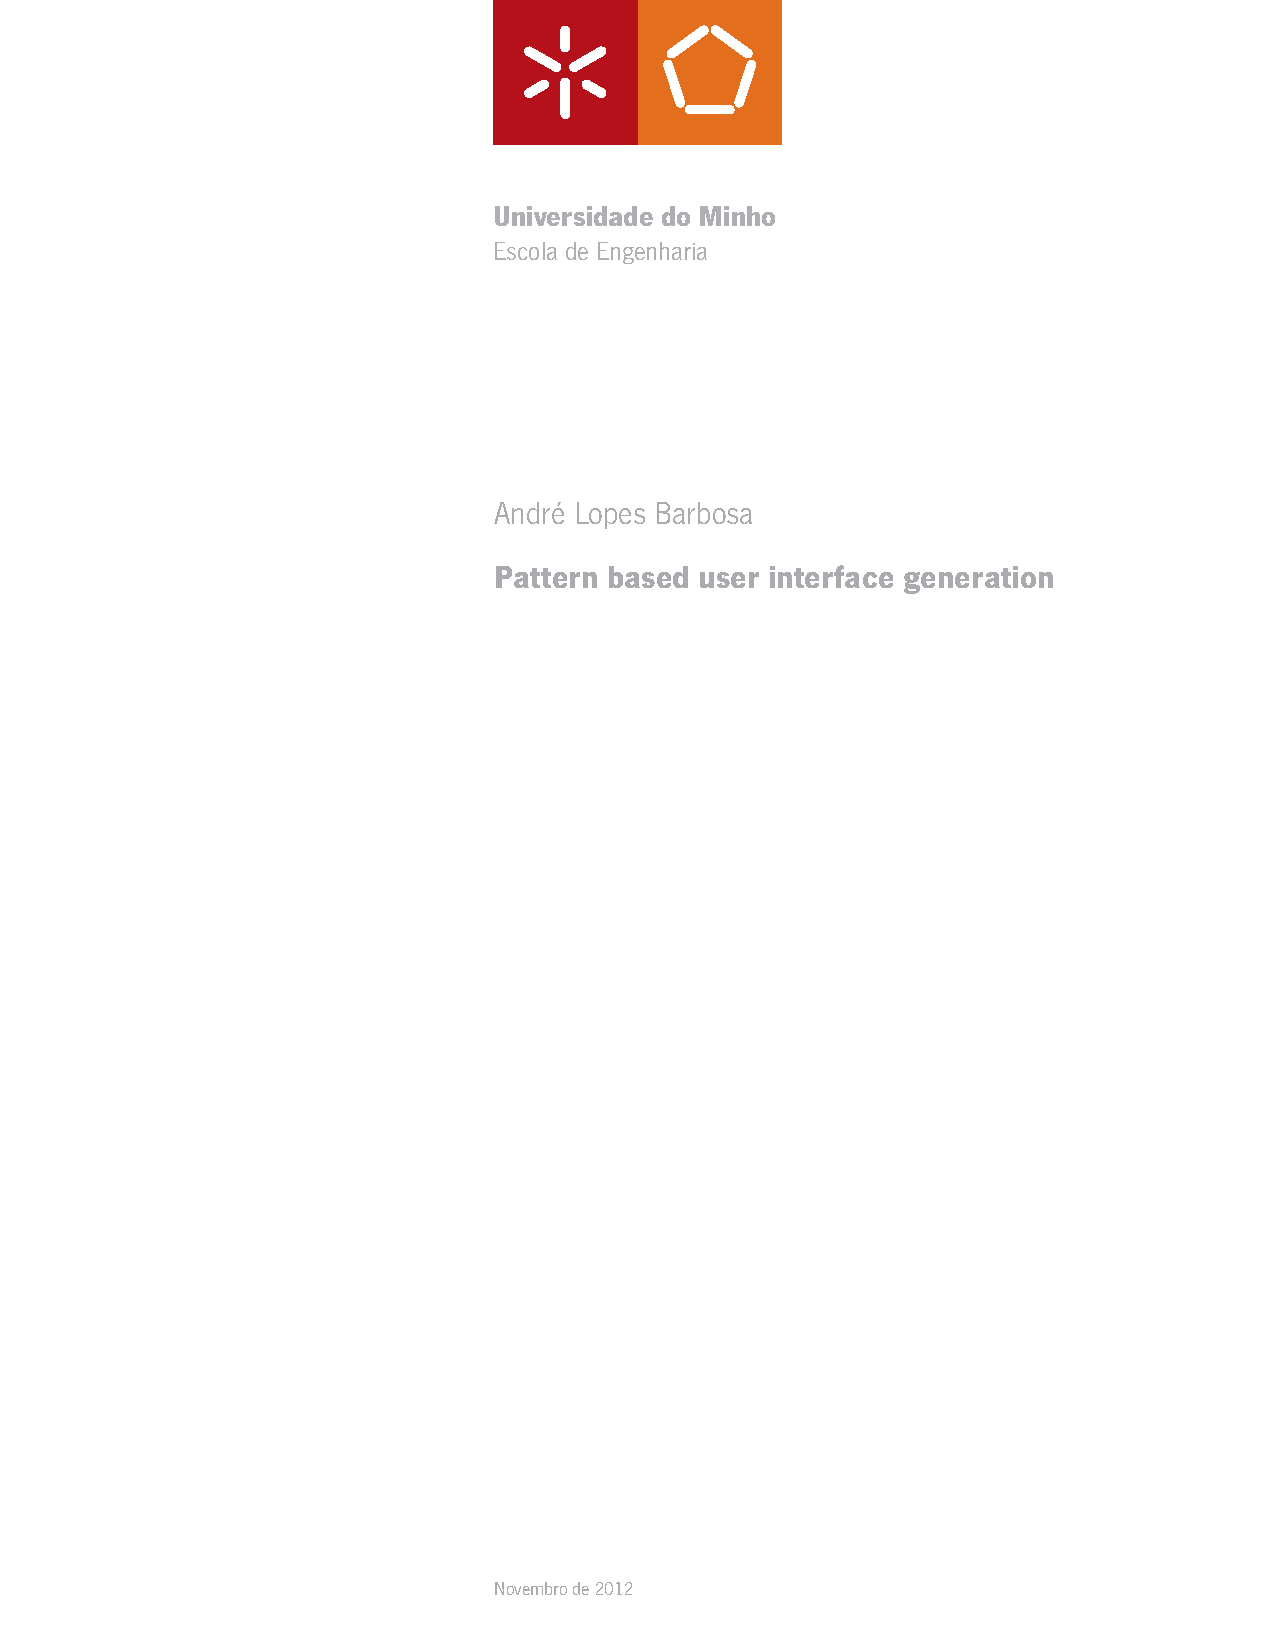
\includepdf[pages=-]{cover/Capa-MIMEI.pdf} 

\pagenumbering{roman}
\setcounter{page}{2}

%%%%%%%%%%%%%%%%%%%%%%%%%%%%%%%%%%%%%%%%%%%%%%%%%%%%%%%%%%

Thank you very much everybody! :D
\cleardoublepage

%%%%%%%%%%%%%%%%%%%%%%%%%%%%%%%%%%%%%%%%%%%%%%%%%%%%%%%%%%

%%%\maketitle
\begin{abstract}
Abstract in english.
\end{abstract}
\cleardoublepage

%%%%%%%%%%%%%%%%%%%%%%%%%%%%%%%%%%%%%%%%%%%%%%%%%%%%%%%%%%

\selectlanguage{portuguese}
%\begin{center}
%\LARGE
%\doublespacing
%Visualização Realista e Interativa de Materiais Complexos
%\normalsize
%\end{center}
%\vspace{15mm}

\begin{abstract}
Resumo em português.
\end{abstract}

\cleardoublepage
\selectlanguage{english}

%%%%%%%%%%%%%%%%%%%%%%%%%%%%%%%%%%%%%%%%%%%%%%%%%%%%%%%%%%

\tableofcontents
%\listoffigures
%\listoftables
\cleardoublepage

\pagenumbering{arabic}
%\setcounter{page}{6}

%%%%%%%%%%%%%%%%%%%%%%%%%%%%%%%%%%%%%%%%%%%%%%%%%%%%%%%%%%


\chapter{State of the art}
In this chapter is described the state art regarding model driven development of user interfaces. It will be presented several techniques to develop user interfaces using model driven principles. There is significant ongoing research in this field since the late 1980s. This chapter makes a short summary of that research. Some works will be examined in more depth for the sake of example. 

Model driven development defining characteristic is that software development's primary focus and products are models rather than computer programs. The major advantage of this is that we express models using concepts that are much less bound to the underlying implementation technology and are much closer to the problem domain relative to most popular programming languages \cite{The_Pragmatics_of_Model-Driven_Development}.

Models are easier to maintain than the code itself and, most importantly, they're platform independent. This means that the same model can be used to generate code that runs on a desktop environment, a web environment or even a mobile environment. This makes a very important feature for user interfaces because modern applications are becoming more and more ubiquitous and it's highly complex and time consuming to build a user interface for every supported platform.

There are different kinds of models and several techniques to model user interfaces. Some tools like Janus\cite{janus} only require a domain model to generate a concrete user interface while others like Trident\cite{trident1, trident2} and Adept\cite{adept1} also use a task model. All these approaches automate part of the development process. Other approaches like ITS\cite{ITS} require more work from the developers because it doesn't generate any model.

Some more recent work have been using different techniques to generate user interfaces. Gadget\cite{gadget} or Supple\cite{supple} have been using optimization techniques to generate better concrete user interfaces

Patterns are widely used in every field of engineering. One of the earlier definitions of patterns can be found on \cite{A_Pattern_Language_Towns_Buildings_Construction}. Almost twenty years later patterns were brought to software engineering by \cite{Design_Patterns}.

Patterns bring many advantages, not only they make the development of a product less time consuming and thus less expensive but can also guarantee a higher level of quality because patterns are solutions that have been tested and used in other projects. IdealXML\cite{IdealXml_An_Interaction_Design_Tool, idealxml2} is a tool that helps developers to take advantage of patterns while developing user interface models.

Although there have been a lot of academic work surrounding model driven development of user interfaces, this work is struggling to be adopted by the industry. There are some theories for what is missing, in \cite{molina} is said that better tool support is needed and in \cite{IdealXml_An_Interaction_Design_Tool} is stated that a common language for representing user interface models is the next step.

UML \cite{The_Unified_Modeling_Language_Reference_Manual} is the industry standard for software modelling but, unfortunately, is not fit to model user interfaces. Fortunately, the software engineering community has developed some new modelling languages in the past few years to overcome this problem. UMLi \cite{User_Interface_Modeling_in_UMLi} is an extension to UML that provides an alternative diagram notation for describing abstract interaction objects. ConcurTaskTrees (CTT) \cite{ConcurTaskTrees_A_Diagrammatic_Notation_for_Specifying_Task_Models} aims at task modelling by dividing the task model is built in three essential parts:
\begin{itemize}
\item First a hierarchical logical decomposition of the tasks represented by a tree-like structure;
\item Then an identification of the temporal relationships among tasks at the same level;
\item And finally an identification of the objects associated with each task and of the actions which allow them to communicate with each other.
\end{itemize} 

UsiXML is a user interface description language aimed at expressing user interfaces built with various modalities of interaction and independently of them. UsiXML is XML compliant to enable flexible exchange of information and powerful communication between models and tools used in user interface engineering \cite{UsiXML_USer_Interface_eXtensible_Markup_Language}. One of the great advantages of UsiXML is platform independence providing a multi-path development of user interfaces \cite{UsiXML_a_Language_Supporting_Multi-Path_Development_of_User_Interfaces}. UsiXML characteristics and features give it the potential to become a standard for modelling user interfaces like UML is for software architecture.

There is a lot of work regarding model driven development for user interfaces and the idea that models can simplify the development process is becoming more consensual. Section \ref{section:early_days} focus on projects from the beginnings of model driven development of user interfaces, namely Janus on section \ref{subsection:janus} and Its, section \ref{subsection:ITS}.

Section \ref{section:optimization_based_generation_of_interfaces} will describe optimization based techniques and the Gadget and Supple projects will be examined with more depth.

Section \ref{section:user_interface_patterns} refers to the usage of patterns in user interface design . This section also includes an analysis of IdealXML, a knowledge based tool for designing user interfaces.

Section \ref{section:specification_languages} is about specification languages. UMLi and UsiXML will be analysed in details in sections \ref{subsection:umli} and \ref{subsection:usixml} respectively.

\section{Early days}
\label{section:early_days}

Research in model-based user interface development comes from the 1980s\cite{SzekelyRetrospective}. Their roots come from user interface management systems (UIMS)\cite{MyersUIMS}. These tools seeked to provide an alternative paradigm for constructing interfaces. Rather than using a toolkit library, developers would write a specification in a specialized, high-level specification language. This specification would be automatically translated into an executable program, or interpreted at run-time to generate the appropriate interface.

Through the 1980s and 1990s the specification languages became more sophisticated, supporting richer and more detailed representations that allowed the systems to generate more sophisticated interfaces.

Since that time there were essentially two approaches to model driven development of user interfaces. Some tried to minimize the work of developers and generate most of the model from just a domain model like in JANUS\cite{janus} or a task model as in TRIDENT\cite{trident1, trident2}. The second approach was to give more power to the developer letting him produce all or most of the model like in ITS\cite{ITS}.

This section includes a more in depth study of one project from each category. On section \ref{subsection:janus} the JANUS project and on section \ref{subsection:ITS} ITS.

\subsection{Janus}
\label{subsection:janus}
\subsection{ITS}
\label{subsection:ITS}
The Its\cite{ITS} system was developed in the early 90s by the IBM research and development department. It was successfully used to develop several large applications like the information kiosks for Seville Expo 92.

The Its architecture divides applications in four layers. The action layer implements the application's back-end computations. The dialogue layer defines the content of the user interface independent of its style, much like an abstract user interface model. Content specifies the objects included in each frame of the interface, the flow of control among frames, and what actions are associated with each object. The style rule layer defines how the dialogue is presented to the user in terms of appearance and interaction techniques. Finally the style program layer implements the primitive tool-kit objects that are composed by the rule layer into complete interaction techniques.

Before Its came along there were mainly two types of layered architectures that provided the required flexibility in application development. User Interface Management Systems (UIMS) and tool-kits. UIMS separate the business layer from the interface. Back-end computations are separated from the dialogue control and style. Style, however, was often treated in a single interface layer. Tool-kits separated style from the application. Dialogue control remained in the back-end while the implementation of interaction techniques is hidden in a code library.

The four layers in Its present a series of advantages that separate this tool from its predecessors. Like in previous UIMS there is a separation from back-end computations and the interface itself. By separating the action layer from the dialogue allows actions to be reused in different applications.

Splitting the interface into separate layers for style-independent dialogue, rule base and tool-kit also gives some benefits. First, the dialogue remains independent of style. A dialogue can be mapped into any different style simply by firing the appropriate rule. Second, interface designers control style rather than application programmers. The rule layer represents the selection criteria for all interaction techniques.

Each layer in Its architecture corresponds to one of four roles in application development: application programmer, application expert, style expert and style programmer. An application expert is familiar with the domain of the application. The application expert typically is neither trained in software development or part of an information systems department. In Its, the application expert is the author of the dialogue. A style expert may be a graphic artist or a human factors engineer. Rules give them direct control over style in Its.

Its is a specification-based system. The main difference between these tools from automated-design tools like Janus\cite{janus} is that the modelling language is open whereas in automated-design tools are closed. By lifting this limitation for the developers the final result can have a higher level of quality although it's dependent from the capabilities of the developer himself.

Even though Its is a specification-based system, this doesn't mean that developers have to specify every feature of every individual window. Developers are forced to specify the content of dialogues which is equivalent to the abstract user interface and this is, as been proved to be by experience, the most difficult model to generate by the automated-design tools. The style rules layer or the concrete user interface model doesn’t have to be totally specified. This doesn’t mean that ITS generates this model but that developers can reuse rule sets from libraries that contain the abstract to concrete mapping for significant portions of the interface specifications.

\section{Optimization-based generation of interfaces}
\label{section:optimization_based_generation_of_interfaces}

Recent work is beginning to reveal that numerical optimization can play a role on modern approaches for generating interfaces and displays. Gadget\cite{gadget} and Supple\cite{supple} are two examples of this tendency.

The first is a framework that aims to provide developers with none or few knowledge on numerical optimization a set of tools that allows them to generate user interfaces through optimization methods.

The second is a tool that aims the generation of personalized user interfaces at run time. The main motivation behind Supple is that current user interfaces are developed with only a limited set of user abilities in mind leaving people with special needs with difficulties to interact with their applications.

\subsection{GADGET}
\label{subsection:GADGET}

Although optimization-based techniques appear to offer several potential advantages most programmers are intimidated or uncomfortable by the math required to program an optimization. Although optimization tool-kits are available (cite), they typically require substantial specialized knowledge because they have mostly been designed for physics simulations and other traditional optimization problems.

GADGET provides a set of abstractions for many optimization concepts along with a set of mechanisms to help programmers quickly create optimizations, including an efficient lazy evaluation framework, a powerful and configurable optimization structure, and a library of reusable components.
A programmer creating an optimization using the GADGET tool-kit needs to supply three essential components: an initializer, iterations and evaluations. The initializer creates the initial solutions to be optimized. This might be based on an existing algorithm, or done randomly. Iterations are responsible to transform one potential solution into another, typically using models that are at least partially random. Finally, evaluations are used to judge the different notions of goodness in a solution.

There’s a standard framework to abstract the concepts and constructs behind evaluations. GADGET allows programmers to focus on creating evaluations to measure criteria that are important to a problem. GADGET then combines these evaluations and uses them to between possible solutions to a problem. This process is divided into five stages. 

First the framework presents each evaluation with the current potential solution, which is called the prior solution. Each evaluation returns an array of double values representing its interpretation of the prior solution. This collection of arrays of double values is called the prior result. 

On the second stage the framework uses an iteration object to modify the prior solution and create a new one, called the post solution.

Third, the framework presents the post solution to each evaluation. Each individual evaluation returns interpretations that are then combined to create a post result.

In the fourth step, the framework uses a method to compare the prior result with the post result. This is possible by requiring each evaluation to be capable of comparing two arrays of double values that it has created and providing a double value in the range of $-1$ to $1$, where $-1$ indicates the evaluation has a strong preference for the prior solution, $0$ indicates that the evaluation is indifferent and 1 indicates that the evaluation has a strong preference for the post solution.

Finally, the result of this comparison indicates whether the framework should go with the post solution or revert to the prior solution. To choose between them, the values retrieved from the fourth step are multiplied by the weight associated with its respective evaluation and then summed. If the sum is greater than 0, the framework prefers the post solution, else it reverts to the prior solution. 
\subsection{Supple}
\label{subsection:Supple}

\section{User interface patterns}
\label{section:user_interface_patterns}

Patterns are widely used in every field of engineering. One of the earlier definitions of patterns can be found on \cite{A_Pattern_Language_Towns_Buildings_Construction}. Almost twenty years later patterns were brought to software engineering by \cite{Design_Patterns}.

Patterns bring many advantages, not only they make the development of a product less time consuming and thus less expensive but can also guarantee a higher level of quality because patterns are solutions that have been tested and used in other projects.

Particularly on user interfaces, these are very important features because building a good user interface is a very complex and time consuming process. On most software projects it takes about half of the time frame allocated to that project, so patterns can help to make this process more efficient. Also there's the problem of usability. This is one of the most important aspects of software projects but its still very difficult to build a user interface compliant with human computer interaction (HCI) rules. By using patterns this can be easily achieved if the patterns are already compliant with these rules.

Patterns are usually stored in catalogues. In \cite{Design_Patterns} a pattern is composed by the following fields:
\begin{itemize}
\item The \textbf{Pattern name} resumes the pattern in one or two words that we use to refer to named pattern.
\item The \textbf{Problem} describes in which situations the pattern should be applied.
\item The \textbf{Solution} describes how the pattern works, what elements it has and how they relate to each other.
\item The \textbf{Consequences} describe the side effects of using the pattern.
\end{itemize}
This is the specification used for software design patterns but it's also used in most user interface patterns catalogs.
In \cite{Generative_pattern-based_design_of_user_interfaces} documentation of patterns is divided in two categories, descriptive patterns and generative patterns. Descriptive patterns are meant to be interpreted by humans so they describe the solution in a generic way so that the pattern can be used in a wide range of contexts while generative patterns maximize \textit{expressivity} over \textit{genericity} thus, they can be used in more restricted range of contexts but the solution is specific enough to be interpreted by machines. 

Design patterns like the ones described in \cite{Design_Patterns} are generative patterns because their solution is specified in UML which is a formal language that can be easily interpreted by machines to perform transformations.

A list of catalogues for user interfaces can be found in \cite{The_Interaction_Design_Patterns_Page}. Most of these catalogues define their solutions with text and images because there isn't a reference language to specify user interfaces. Thus most of these patterns are descriptive patterns that can only be used by humans.

In order to take full advantage of patterns we need a way to document them. Generative patterns are the most useful in the context of this project but to use them we need to find a language to specify these patterns so that they can be interpreted by a machine to generate a concrete user interface. applications. In section \ref{subsection:IdealXML} is described IdealXML a tool for developing user interface models that takes advantages of patterns.

\subsection{IdealXML}
\label{subsection:IdealXML}

IdealXML\cite{IdealXml_An_Interaction_Design_Tool, idealxml2} is an experience-based environment for user interface design. Experience is the accumulation of knowledge or skills that result from direct participation in events or activities. Developers have a strong tendency to towards reusing designs that worked well for them in the past. Unfortunately, this design reuse is usually limited by personal experience, and there is usually few sharing of knowledge among developers.

IdealXML manipulates a pattern repository, where patterns are organized following a hierarchical structure. At the top, this structure has different models related with a MB-UIDE: domain, task, presentation and mapping, context and user models are left for future work. IdealXML is shipped with a predefined collection of patterns from a variety of sources. These patterns are the initial base of knowledge.

IdealXML is an MB-UIDE and designers can, using several graphical notations, specify domain models, task models, abstract presentation models and mapping models between them. Some of these models are stored in the pattern repository and new ones can always be added.

IdealXML also allows for the animation of a task model to generate a hi-fi prototype of the future user interface while still in the first development stages. This is achieved by using CTT, UsiXML and a set of heuristics to transform the task model specification into an abstract UI.

Prototyping consists in the creation of a preliminary version of the future UI (prototype) so that the user and the experts can find possible problems in the design of the UI, both from the functional and from the usability points of view. Prototyping techniques fall into two main categories:
\begin{itemize}
\item \textbf{Lo-fi:} this family of techniques is mostly used in requirements analysis stage to validate the requirements with the user in user-centred approaches.

\item \textbf{Hi-fi:} they are aimed at the creation of preliminarily versions of the UI with an acceptable degree of quality. This kind of techniques produces a UI prototype which is closer to final future one.
\end{itemize}

Abstract prototyping was devised because it was found that the sooner developers started drawing realistic pictures or positioning real widgets, the longer it took them to converge on a good design.

As it was mentioned above, IdealXML uses a set of heuristics to transform the task model into an abstract interface model:
\begin{itemize}
\item Each cluster of interrelated task cases becomes an interaction space in the navigation map, so an abstract task is a container.
\item A container also can be an interaction task or an application task in a hierarchical task decomposition.
\item A component rises when an interaction or application task is found in a hierarchical task decomposition.
\item A component can have several facets (input, output, control and navigation). These facets allow the user to interact with the system.
\end{itemize}

The animation of the abstract user interface that resulted from the designed task model is grounded in the identification of the enabled task set (ETS). Having identified the ETC for a task model, the next step is to identify the effects of performing each task in each ETS. The result of this analysis is  a state and transitions occur when tasks are performed. In IdealXML's proposal, the task model specification is split into states. Each state is a set of interrelated tasks, including temporal relationships between those tasks, usually connected to an essential use case.
\section{Specification languages}
\label{section:specification_languages}

In \cite{idealxml2} was stated that one of the most important challenges to overcome in model driven development of user interfaces is the creation of a specification language that would be massively adopted and became a common ground between developers like UML is for software architecture.

Over the years many languages were developed to try and overcome this obstacle. In \cite{mecano} were enumerated some of the problems found with that time user interface models:
\begin{itemize}
\item \textbf{Partial models}, most models deal only with a portion of the spectrum of interface characteristics. Some emphasize domain, others emphasize tasks, some others emphasize presentation guidelines and so on.

\item \textbf{Insufficient underlying model}, several model-based systems use modelling paradigms proven successful in other applications areas, but that come up short for interface development. These underlying models typically result in partial interface models of restricted expressiveness.

\item \textbf{System-dependent models}, many interface models are non-declarative and are embedded implicitly into their associated model-based systems, sometimes at code level. These generic models are tied to the interface generation schema of their system, and are therefore unusable in any other environment.

\item \textbf{Inflexible models}, experience with model-based systems suggests that interface developers often wish to change, modify, or expand the interface model associated with a particular model-based environment. However, model-based systems do not offer facilities to such modifications, nor the interface models in question are defined in a way that modifications can be easily accomplished. Thus the inclusion of an open meta-model like in UML could be an important factor of success.
\end{itemize}

Next, two recent specification languages for user interfaces that try to overcome these problems will be presented. In section \ref{subsection:umli} will be presented UMLi, an extension to UML to support the modelling of user interfaces. In section \ref{subsection:usixml} will be presented UsiXML, a language with potential to become a standard in user interface specification.

\subsection{UMLi}
\label{subsection:umli}


\subsection{UsiXML}
\label{subsection:usixml}

UsiXML (USer Interface eXtensible Markup Language) is a User Interface Description Language (UIDL) that uses Model-Driven Engineering (MDE) for specifying a User Interface (UI) at an implementation independent level. The UI specifications are usually specified in different models. Each UI level is described by a model(s). UsiXML is based on the Cameleon reference framework\cite{Calvary}. This framework describes a UI in four main levels of abstraction: task and domain level, abstract UI level, concrete UI and final UI. On the basis of these 4 levels, UsiXML proposes a set of models:
\begin{itemize}
\item \textbf{Transformation model}: contains a set of rules in order to enable a transformation of one specification to another.
\item \textbf{Domain model}: describes the classes of the objects manipulated by the users while interacting with the system.
\item \textbf{Task model}: describes the interactive task as viewed by the user interacting with the system. The task model is expressed according to the CTT specification \cite{ConcurTaskTrees_A_Diagrammatic_Notation_for_Specifying_Task_Models}.
\item \textbf{Abstract user interface model}: represents the view and behavior of the domain concepts and functions in platform independent way.
\item \textbf{Concrete user interface model}: represents a concretization of the abstract user interface model.
\item \textbf{Mapping model}: contains a series of related mappings between models or elements of models.
\item \textbf{Context model}: describes the three aspects of a context of use, which is a user carrying out an interactive task using a specific computing platform in a given surrounding environment.
\item \textbf{Resource model}: contains definitions of resources attached to abstract or concrete interaction objects.
\end{itemize}

The user interface model in UsiXML consists of a list of component models (described above) in any order and any number. It doesn't need to include one of each model component and there can be more than one of a particular kind of model component. It's also composed by a creation date, a list of modification dates, a list of authors and a schema version.

UsiXML allows designers to apply a multi-path development of user interfaces. In this development paradigm, a user interface can be specified and produced at and from different, and possibly multiple, levels of abstraction while maintaining the mappings between these levels if required. Thus, the development process can be initiated from any level of abstraction and proceed towards obtaining one or many final user interfaces for various contexts of use at other levels of abstraction. In this way, the model-to-model transformation, which is the cornerstone of Model-Driven Architecture (MDA), can be supported in multiple configurations, based on composition of three basic transformation types\cite{UsiXML_a_Language_Supporting_Multi-Path_Development_of_User_Interfaces}:
\begin{itemize}
\item \textbf{abstraction}, is the process of substitution of the input artefacts into more abstract ones;
\item \textbf{reification}, is the process of substitution of the input artefacts into more concrete ones;
\item \textbf{translation}, is the process of substitution of the input artefacts aimed at a particular context of use into others that are aimed for a different context.
\end{itemize} 


Multi-path UI development is based on the Cameleon Reference Framework\cite{Calvary}, which defines UI development steps for multi-context interactive applications. The development process with this framework is structured in four steps where each developments step is able to manipulate a set of artefacts in the form of models:
\begin{itemize}
\item \textbf{Final UI (FUI)}: is the operational UI. Any UI running on a particular computing platform either by interpretation or by execution.

\item \textbf{Concrete UI (CUI)}: it's a transformation of the abstract UI for a given context of use into Concrete Interaction Objects (CIOs). It defines widgets layout and interface navigation. The CUI abstracts a FUI into a UI definition that is independent of any computing platform. Although a CUI makes explicit the final appearance and style of a FUI, it is still a mock-up that runs only within a particular environment. A CUI can also be considered as a reification of an AUI at the upper level and an abstraction of the FUI with respect to the platform.

\item \textbf{Abstract UI (AUI)}: defines interaction spaces by grouping subtasks according to various criteria, a navigation scheme between the interaction spaces and selects Abstract Interaction Objects (AIOs) for each concept so that they are independent of any modality. An AUI abstracts a CUI into a UI definition that is independent of any modality of interaction. An AUI can also be considered as a canonical expression of the rendering of the domain concepts and tasks in a way that is independent from any modality of interaction. An AUI is considered as an abstraction of a CUI with respect to modality.

\item \textbf{Task and Domain (T\&D)}: describe the various tasks to be carried out and the domain-oriented concepts as they are required by these tasks to be performed. These objects are considered as instances of classes representing the concepts manipulated.
\end{itemize}

UsiXML is also very extensible. At the model level USIXML allows to define any kind of model. In this sense it is possible to instantiate any new model of the above mentioned classes. At meta-model level USIXML offers a modular structure which clearly segregates the models it describes. This facilitates the integration of new classes of models into UsiXML. The model and its concept is simply declared along with its relationships with other models. Rules exploiting this new model can be defined afterwards.

In conclusion, UsiXML solves every problem stated in \cite{mecano}. UsiXML was design for user interfaces, it's not and adaptation of some modelling language that was meant for other use. It provides several classes of models with different abstraction levels so that every part of the interface is specified. By allowing the application of multi-path development process, it makes sure that every specification is platform independent. Finally, it's a flexible language, UsiXML provides mechanisms that can be used to extend and modify it's models and transformation rules.

\section{Conclusion}

The first tools in this chapter were Janus\cite{janus} and Its\cite{ITS}. These tools represent the beginning of model driven development of user interfaces and at the same time two different approaches to this subject. Developers using Janus will decrease the development time of their applications. This seems to be the main goal of the project. Because it only needs one input, the domain model, it doesn't take a lot of effort to create a user interface. Of course this also means that the generated user interface won't have the same quality as one built by hand (depending on the abilities of the developer) and this is the most criticized aspect of Janus. On the other hand, Its can produce high quality user interfaces. But the amount of work necessary to build something is huge compared to Janus. Its also provides a way to divide work through the development team which is a very interesting feature because it facilitates the implementation of different development methodologies alongside this tool.

By analysing these two projects one can infer that there model driven development can be used with two objectives in mind:
\begin{enumerate}
\item to build low-cost prototypes of an application rapidly;
\item to enhance the quality of the final product.
\end{enumerate}

Janus is clearly a tool that can be used to rapidly create a prototype of an in development application that can be used to communicate with customers or other stake holders. Its is aimed at building better applications with large teams.


\subsection{UsiXML}
\label{subsection:usixml}

UsiXML (USer Interface eXtensible Markup Language) is a User Interface Description Language (UIDL) that uses Model-Driven Engineering (MDE) for specifying a User Interface (UI) at an implementation independent level. The UI specifications are usually specified in different models. Each UI level is described by a model(s). UsiXML is based on the Cameleon reference framework\cite{Calvary}. This framework describes a UI in four main levels of abstraction: task and domain level, abstract UI level, concrete UI and final UI. On the basis of these 4 levels, UsiXML proposes a set of models:
\begin{itemize}
\item \textbf{Transformation model}: contains a set of rules in order to enable a transformation of one specification to another.
\item \textbf{Domain model}: describes the classes of the objects manipulated by the users while interacting with the system.
\item \textbf{Task model}: describes the interactive task as viewed by the user interacting with the system. The task model is expressed according to the CTT specification \cite{ConcurTaskTrees_A_Diagrammatic_Notation_for_Specifying_Task_Models}.
\item \textbf{Abstract user interface model}: represents the view and behavior of the domain concepts and functions in platform independent way.
\item \textbf{Concrete user interface model}: represents a concretization of the abstract user interface model.
\item \textbf{Mapping model}: contains a series of related mappings between models or elements of models.
\item \textbf{Context model}: describes the three aspects of a context of use, which is a user carrying out an interactive task using a specific computing platform in a given surrounding environment.
\item \textbf{Resource model}: contains definitions of resources attached to abstract or concrete interaction objects.
\end{itemize}

The user interface model in UsiXML consists of a list of component models (described above) in any order and any number. It doesn't need to include one of each model component and there can be more than one of a particular kind of model component. It's also composed by a creation date, a list of modification dates, a list of authors and a schema version.

UsiXML allows designers to apply a multi-path development of user interfaces. In this development paradigm, a user interface can be specified and produced at and from different, and possibly multiple, levels of abstraction while maintaining the mappings between these levels if required. Thus, the development process can be initiated from any level of abstraction and proceed towards obtaining one or many final user interfaces for various contexts of use at other levels of abstraction. In this way, the model-to-model transformation, which is the cornerstone of Model-Driven Architecture (MDA), can be supported in multiple configurations, based on composition of three basic transformation types\cite{UsiXML_a_Language_Supporting_Multi-Path_Development_of_User_Interfaces}:
\begin{itemize}
\item \textbf{abstraction}, is the process of substitution of the input artefacts into more abstract ones;
\item \textbf{reification}, is the process of substitution of the input artefacts into more concrete ones;
\item \textbf{translation}, is the process of substitution of the input artefacts aimed at a particular context of use into others that are aimed for a different context.
\end{itemize} 


Multi-path UI development is based on the Cameleon Reference Framework\cite{Calvary}, which defines UI development steps for multi-context interactive applications. The development process with this framework is structured in four steps where each developments step is able to manipulate a set of artefacts in the form of models:
\begin{itemize}
\item \textbf{Final UI (FUI)}: is the operational UI. Any UI running on a particular computing platform either by interpretation or by execution.

\item \textbf{Concrete UI (CUI)}: it's a transformation of the abstract UI for a given context of use into Concrete Interaction Objects (CIOs). It defines widgets layout and interface navigation. The CUI abstracts a FUI into a UI definition that is independent of any computing platform. Although a CUI makes explicit the final appearance and style of a FUI, it is still a mock-up that runs only within a particular environment. A CUI can also be considered as a reification of an AUI at the upper level and an abstraction of the FUI with respect to the platform.

\item \textbf{Abstract UI (AUI)}: defines interaction spaces by grouping subtasks according to various criteria, a navigation scheme between the interaction spaces and selects Abstract Interaction Objects (AIOs) for each concept so that they are independent of any modality. An AUI abstracts a CUI into a UI definition that is independent of any modality of interaction. An AUI can also be considered as a canonical expression of the rendering of the domain concepts and tasks in a way that is independent from any modality of interaction. An AUI is considered as an abstraction of a CUI with respect to modality.

\item \textbf{Task and Domain (T\&D)}: describe the various tasks to be carried out and the domain-oriented concepts as they are required by these tasks to be performed. These objects are considered as instances of classes representing the concepts manipulated.
\end{itemize}

UsiXML is also very extensible. At the model level USIXML allows to define any kind of model. In this sense it is possible to instantiate any new model of the above mentioned classes. At meta-model level USIXML offers a modular structure which clearly segregates the models it describes. This facilitates the integration of new classes of models into UsiXML. The model and its concept is simply declared along with its relationships with other models. Rules exploiting this new model can be defined afterwards.

In conclusion, UsiXML solves every problem stated in \cite{mecano}. UsiXML was design for user interfaces, it's not and adaptation of some modelling language that was meant for other use. It provides several classes of models with different abstraction levels so that every part of the interface is specified. By allowing the application of multi-path development process, it makes sure that every specification is platform independent. Finally, it's a flexible language, UsiXML provides mechanisms that can be used to extend and modify it's models and transformation rules.
%\chapter{Requirements}

\newcommand{\mh}{\hl{Must Have}}
\newcommand{\sh}{\hl{Should Have}}
\newcommand{\ch}{\hl{Could Have}}
\newcommand{\wh}{\hl{Won't Have}}


%\section{Conclusions}
User interface development is one of the most important phases in software development but still's very hard for developers to manage this process efficiently. The data from section \ref{section:How_user_interfaces_are_built} show's that there is a need for better tools and methodologies to build user interfaces.

Patterns are very important for engineers, in section \ref{section:Patterns_in_software_engineering} we studied how are patterns used, documented and stored. We divided patterns in two categories, descriptive patterns and generative patterns. Although the ones that are more interesting for this work are generative pattens, there is more abundance of descriptive patters for user interfaces. The main reason for this is the lack of a standard language for specifying user interfaces, like UML for general software.

On section \ref{section:How_to_specify_user_interface_patterns} we studied a couple a languages with the potential to become standard in user interface patterns specification. UsiXML is a more concise language while UsiPXML can store more information in a structured way by merging UsiXML with PLML which is a language for descriptive patterns. In conclusion UsiPXML seems to be more suited to describe patterns but UsiXML is more generic and thus as more potential to become a standard in the software engineering community so it's probably the best option on the table.

The future work for this project will be a more profound study of the UsiXML specification in order to develop a tool capable of reading a pattern described in UsiXML, link it with existing source code (business layer) and generate a concrete user interface.


%%%%%%%%%%%%%%%%%%%%%%%%%%%%%%%%%%%%%%%%%%%%%%%%%%%%%%%%%%

%%%%Bibliography
\bibliography{main}
\bibliographystyle{acm}
%\bibliographystyle{abbrv}
%\bibliographystyle{acmtrans}
%\nocite{*}

\end{document}
